\clearpage
\chapter{B Parking Trigger Strategy}\label{sec:triggers}

The analysis' signal process contains displaced SM $\tau$ leptons in its final state. 
In order to exploit the leptonic decay of $\tau$ lepton with significant IP, specifically with muon final state for clean signal, the B-Parking triggers are used. 
CMS implemented the B-Parking trigger since the year of 2018 of Run 2 for research on lepton universalities. 
As described in chapter \ref{sec:detectors}, lepton universality tests claim that interaction between leptons and a gauge boson measures the same for each lepton. 
In mathematical expression, R(K$^{*}$,D$^{*}$) defined as in formulae \ref{eq:rk} and \ref{eq:rd}, are tested.
\begin{equation}
\label{eq:rk}
	R(K^{*})  = \frac{B->K^{*}\mu^{+}\mu^{-}}{B->K^{*}e^{+}e^{-}} 
\end{equation}
\begin{equation}
\label{eq:rd}
	R(D^{*})  = \frac{B->D^{*}\tau^{\pm}\nu}{B->D^{*}\mu^{\pm}\nu} 
\end{equation}
The first ratio specifically attracts investigation of many physicists.
R(K$^{*}$)'s physics process is highly suppressed due because Flavor-Changing Neutral Current (FCNC) is not allowed in the SM.
For a b-quark to change its flavor to strange quark, it has to go through a loop process with 2 additional vertices, making the cross-section highly suppressed.
Di-muon and di-electron signature of the highly suppressed process is very clean, making it optimal channel to test lepton universality,
Its Feynman diagrams are shown in figures of \ref{fig:LU1} and \ref{fig:LU2} 
\begin{figure}[h!]
  \caption{The figures show two different loop diagrams for B$->K^{*}l^{+}l^{-}$ processes. The FCNC is forbidden in the SM and there is no tree level process for B$->K^{*}l^{+}l^{-}$. Thus, these two processes are the leading contributors for B$->K^{*}l^{+}l^{-}$, which are highly suppressed.}
  \label{fig:LU1}
  \centering
  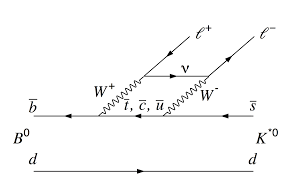
\includegraphics[width=0.57\linewidth]{figs/LU3.png}
  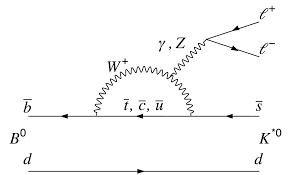
\includegraphics[width=0.57\linewidth]{figs/LU1.png}
\end{figure}
\begin{figure}[h!]
  \caption{If the Lepton universality is not satisfied (R(K$^{*}$,D$^{*} \neq$ 1), it implies there is new physics hidden in the diagram. It could be interpreted in terms of Lepto-quark or Electroweak Z boson which couples to right-hand chrial leptons.}
  \label{fig:LU2}
  \centering
  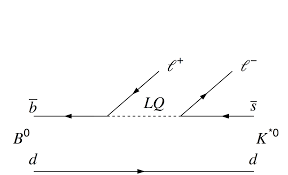
\includegraphics[width=0.57\linewidth]{figs/LU2.png}
  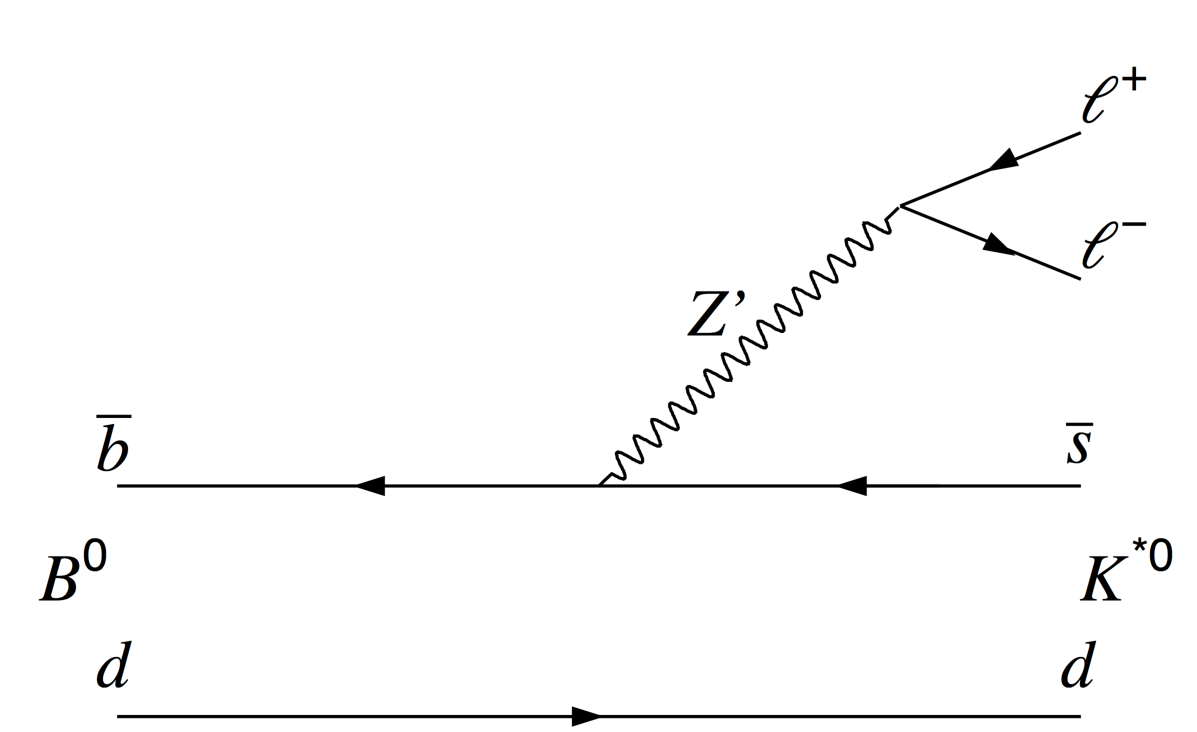
\includegraphics[width=0.57\linewidth]{figs/LU4.png}
\end{figure}
Because of this physics reason, muonic final state of B mesons are desired for research of R(K$^{*}$,D$^{*}$), . 
Consequently, B-parking trigger requires a soft muon with modest displacement (measured using impact parameter) from the primary vertex, as in b-tagging, by exploiting the b-quark's long lifetime.
It requires a muon with transverse momentum (pT) of 7-12 GeV with impact parameter (IP) significance 3-6.

pp collisions in LHC produce extremely enormous amount of events, which could trigger the B parking trigger paths. 
 As discussed in chapter \ref{sec:detector}, Current CPU capacity of CMS is limited and not capable of reconstructing the entire event at such high trigger rate in HLT level.
Thus, CMS scouts events, meaning it writes events that passed L1 trigger to a temporary dataset. Later, full HLT and RECO steps are implemented and served as a B-Parking dataset. 
The prescale factor for BPH triggers is 5-6.


\section{Trigger Paths}
We use data collected by the B-Parking triggers for the year of 2018.
The exact names of paths for B-Parking triggers are listed in Table~\ref{tab:triggers18}.
%We observe that the trigger efficeincy reaches a plateau after requiring a muon with pT value above that utilizes in the L1 seed.
%The standard trigger scale factors are applied in order to correct the MC.

\begin{table}[htb]
\caption{HLT trigger paths used in the analysis 2018.}
\begin{center}
\begin{tabular}{r|l}\hline
\hline
 Data sample & Trigger \\
\hline
 ParkingBPH*-Run2018A & HLT\_Mu9\_IP6\_part* \\
 ParkingBPH*-Run2018B & HLT\_Mu9\_IP6\_part* \\
 \hline
 ParkingBPH*-Run2018C & HLT\_Mu12\_IP6\_part* \\
 ParkingBPH*-Run2018D & HLT\_Mu12\_IP6\_part* \\
 \hline
 \hline
\end{tabular}
\label{tab:triggers18}
\end{center}
\end{table}

\begin{table}[htb]
\caption{Data and MC Global tags used 2018}
\begin{center}
\begin{tabular}{r|l}\hline
 Data 2018 & 106X\_dataRun2\_v29 \\
 \hline
 MC 2018   & 106X\_upgrade2018\_realistic\_v11\_L1v1 \\
 \hline
\end{tabular}
\label{tab:GT}
\end{center}
\end{table}



\begin{figure}[h!]
  \caption{pt of the scalar products}
  \label{fig:scalarpt}
  \centering
  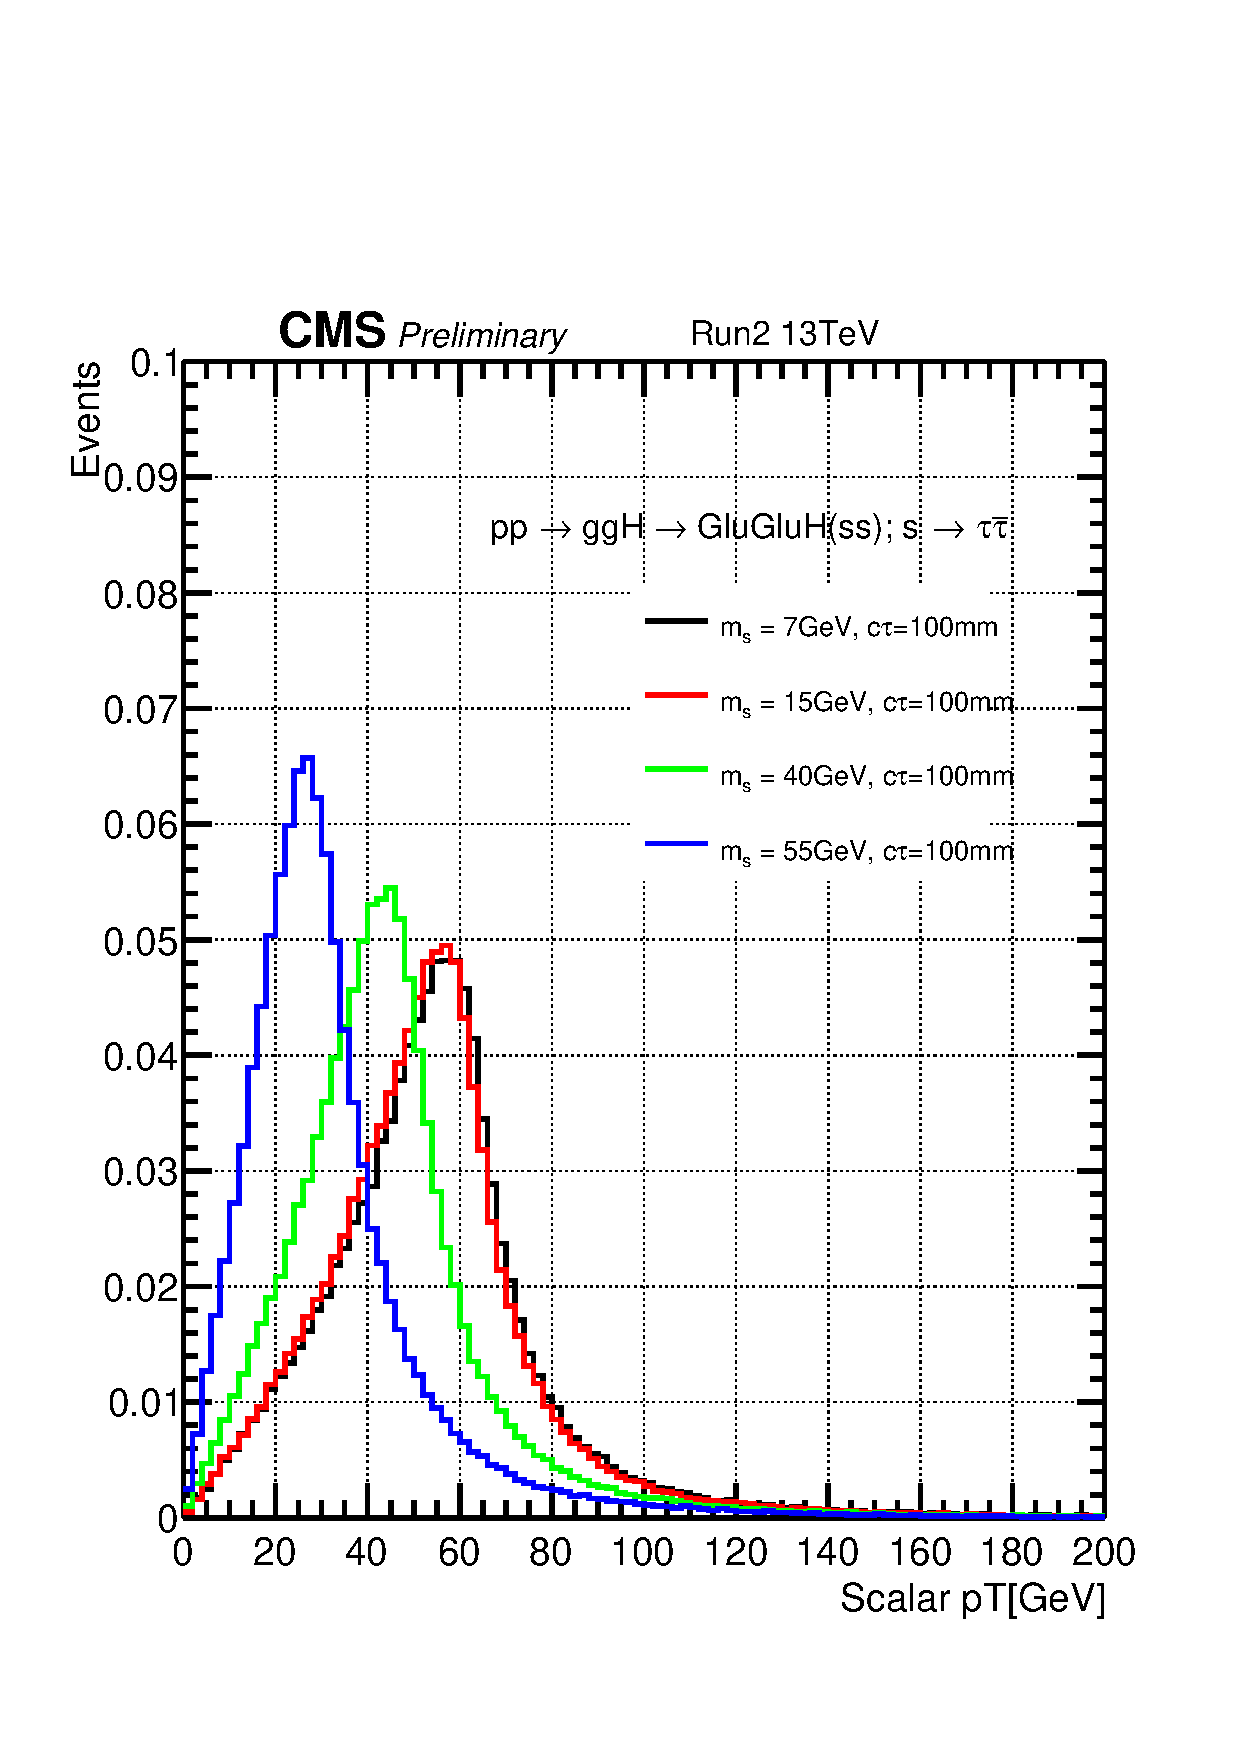
\includegraphics[width=0.5\linewidth]{figs/Scalar_pT100mm.pdf}
\end{figure}

\begin{figure}[h!]
  \caption{DeltaR of the scalar products}
  \label{fig:scalarpt}
  \centering
  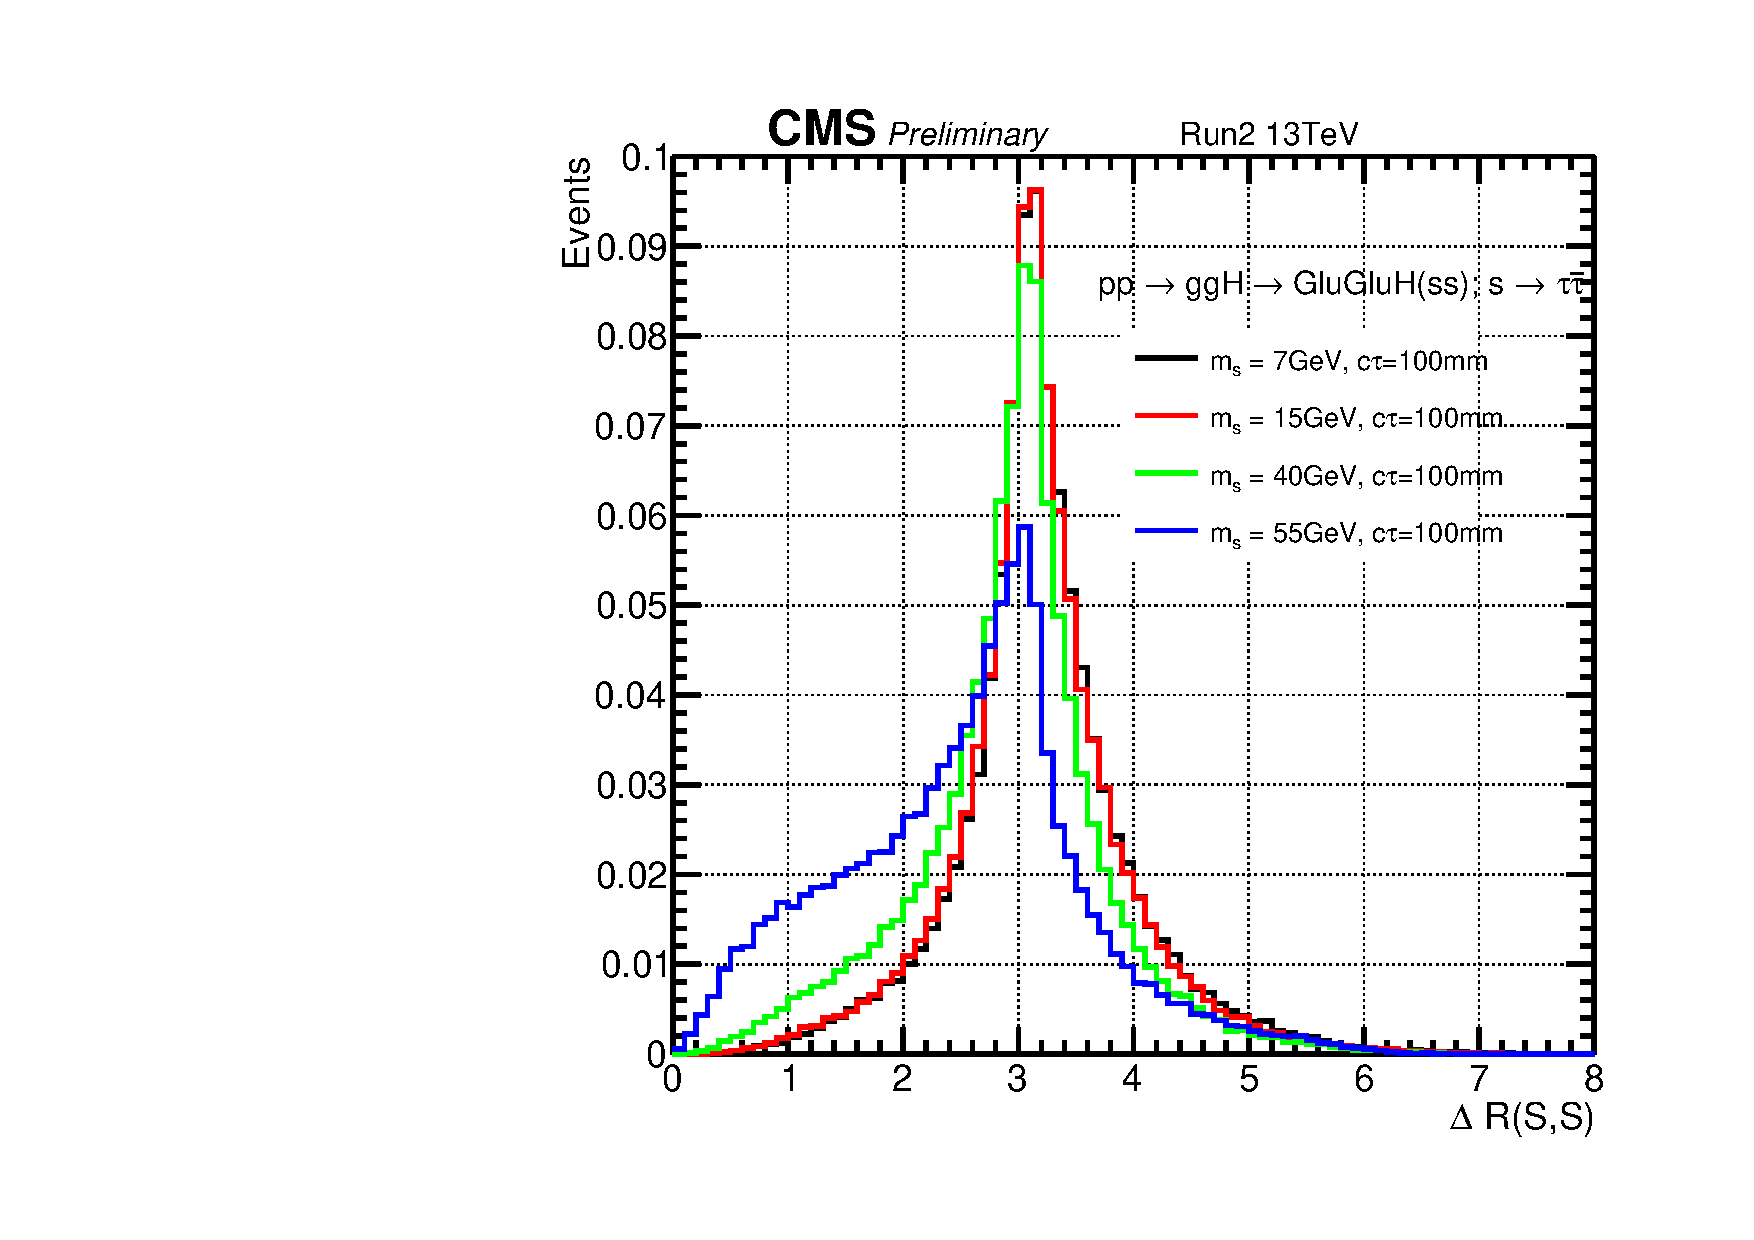
\includegraphics[width=0.5\linewidth]{figs/Scalar_dR100mm.pdf}
\end{figure}

\begin{figure}[h!]
  \caption{liftime of the scalar products in the lab frame}
  \label{fig:scalarpt}
  \centering
  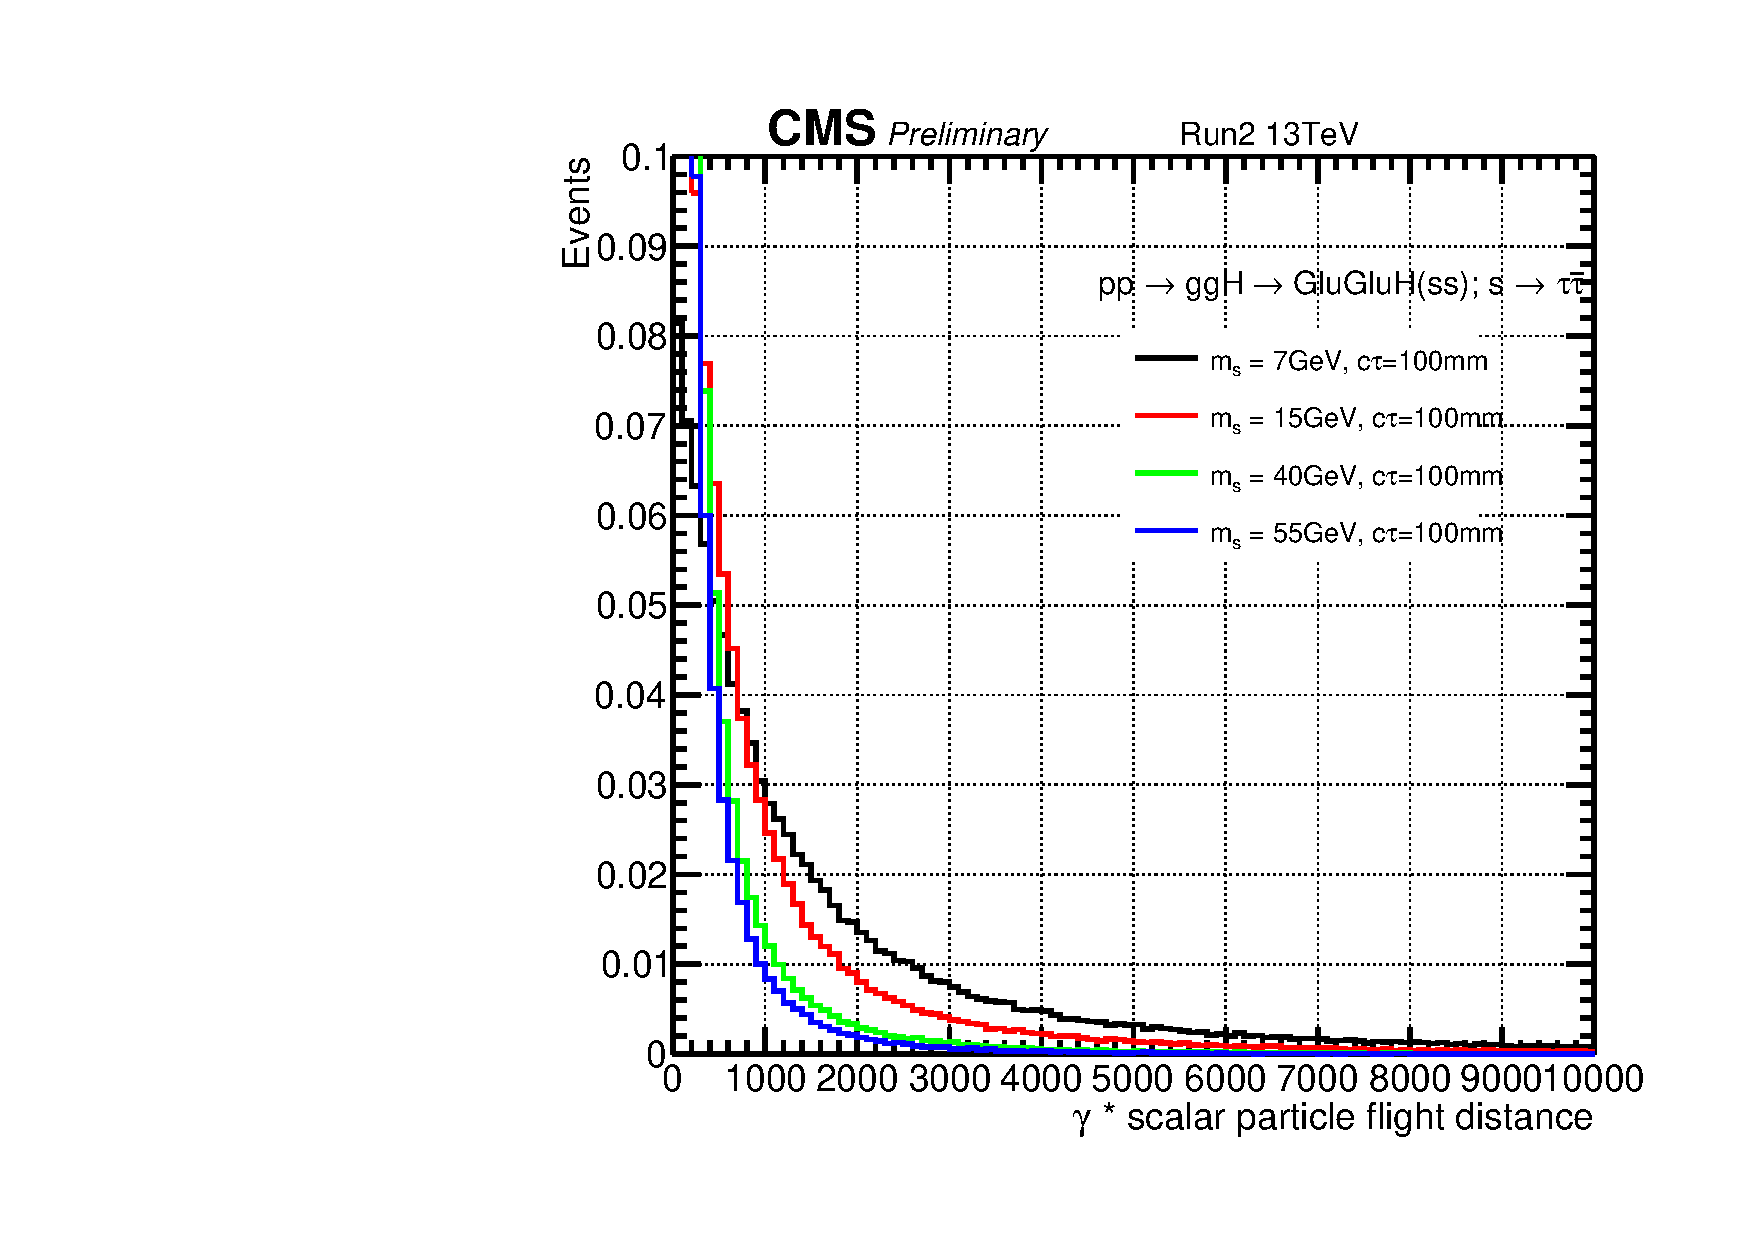
\includegraphics[width=0.57\linewidth]{figs/Scalar_gammactau100mm.pdf}
  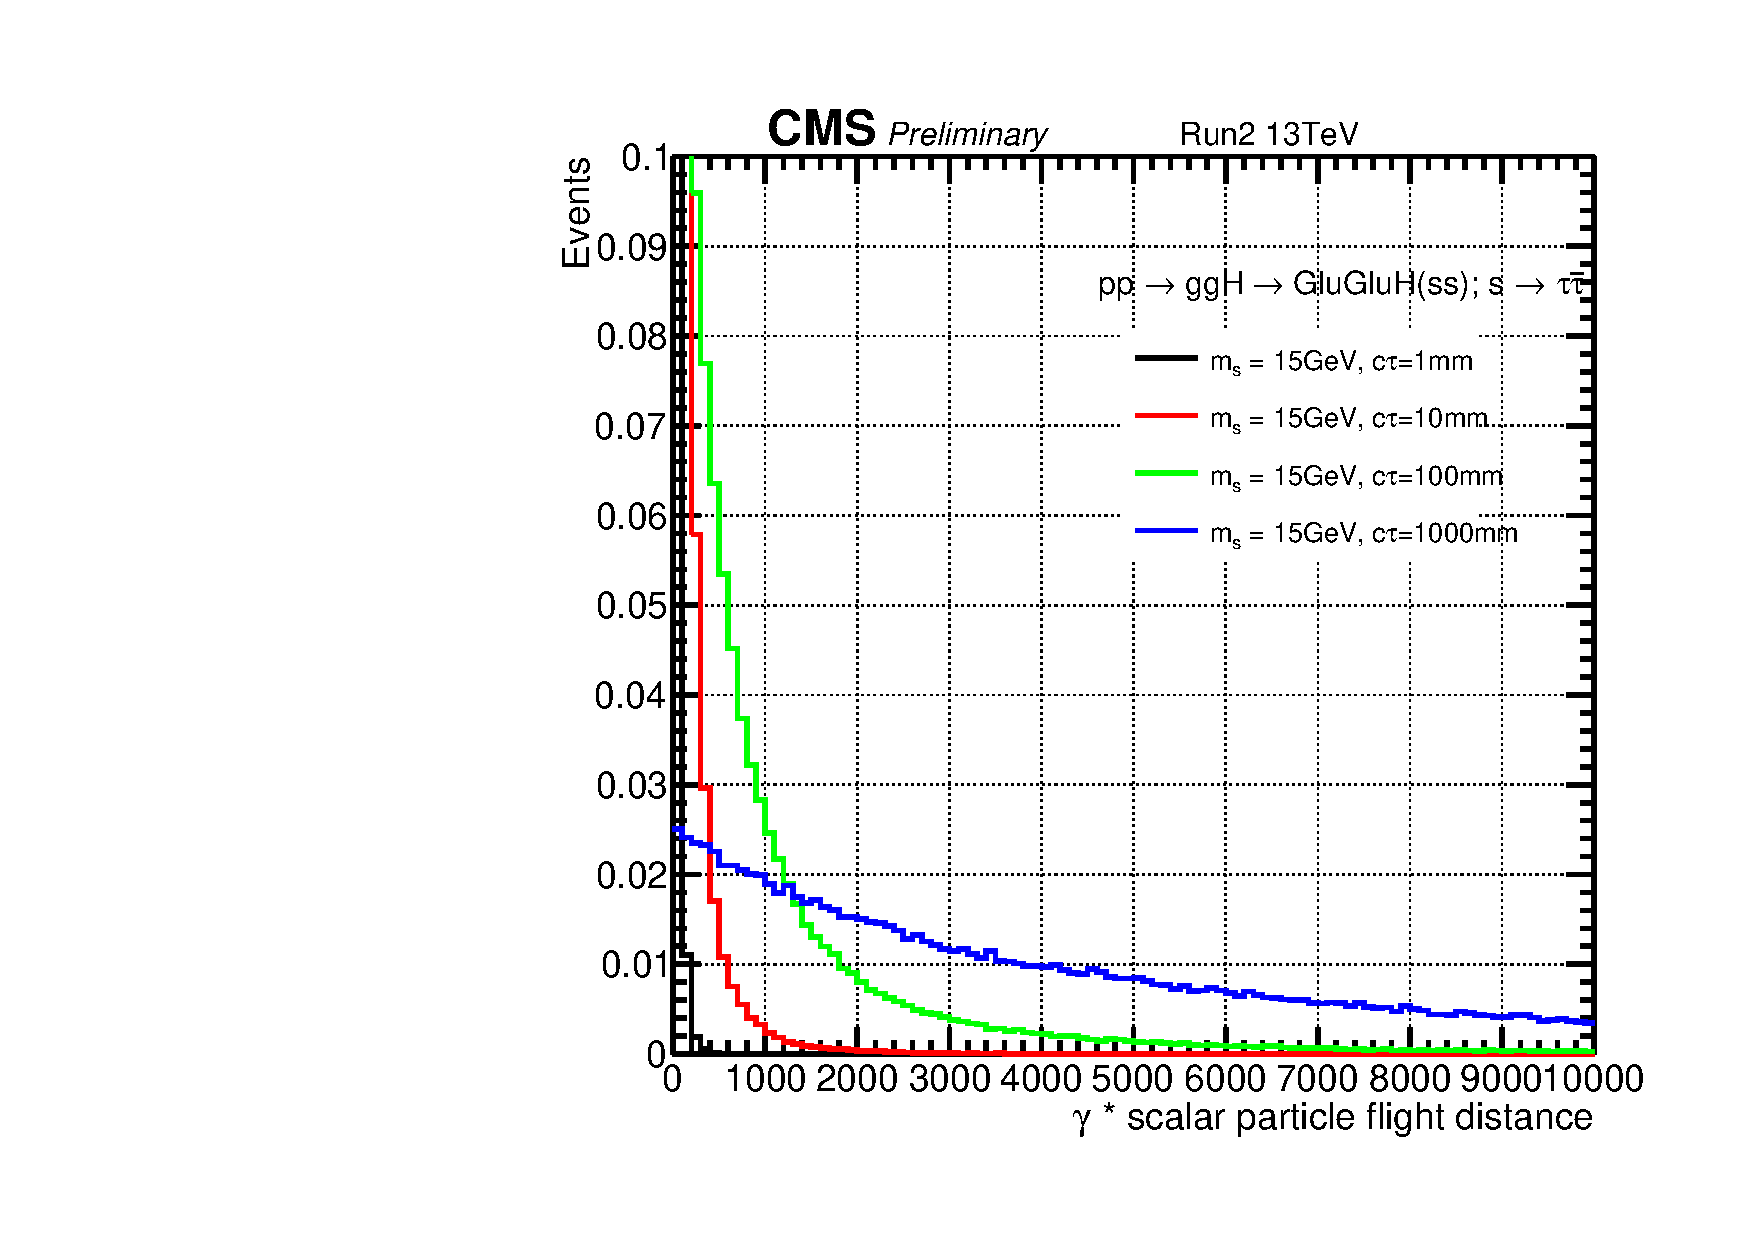
\includegraphics[width=0.57\linewidth]{figs/Scalar_gammactau15GeV.pdf}
\end{figure}


Below is the trigger efficiency of various BPH trigger paths for different mass and lifetime points of the signal (HToSSTo4Tau) sample
Signal process shows an overall good efficiency.
Signal points with LLP's c$\tau$ = 10,100mm show the best performance.
Signal points with LLP's c$\tau$ = 1000mm likely decays outside of the tracker region, leaving no track's impact parameter, and fails to pass the trigger.
On the other hand signal point with LLP's c$\tau$ = 1mm may not reach the first pixel detector, which is at 2.7cm from the beam spot, and fails to pass the trigger.
We can confirm this explanation with observation that lighter LLP's MS has better trigger efficiency for shorter lifetime thanks to higher boost, and the vice versa for heavier LLP's MS. 
\begin{figure}[h!]
  \caption{The plots show the trigger efficiency for each HLT path with respect to LLP's lifetime. Each line denotes mass scale of each scalar.}
  \label{fig:Trigger Efficiency}
  \centering
  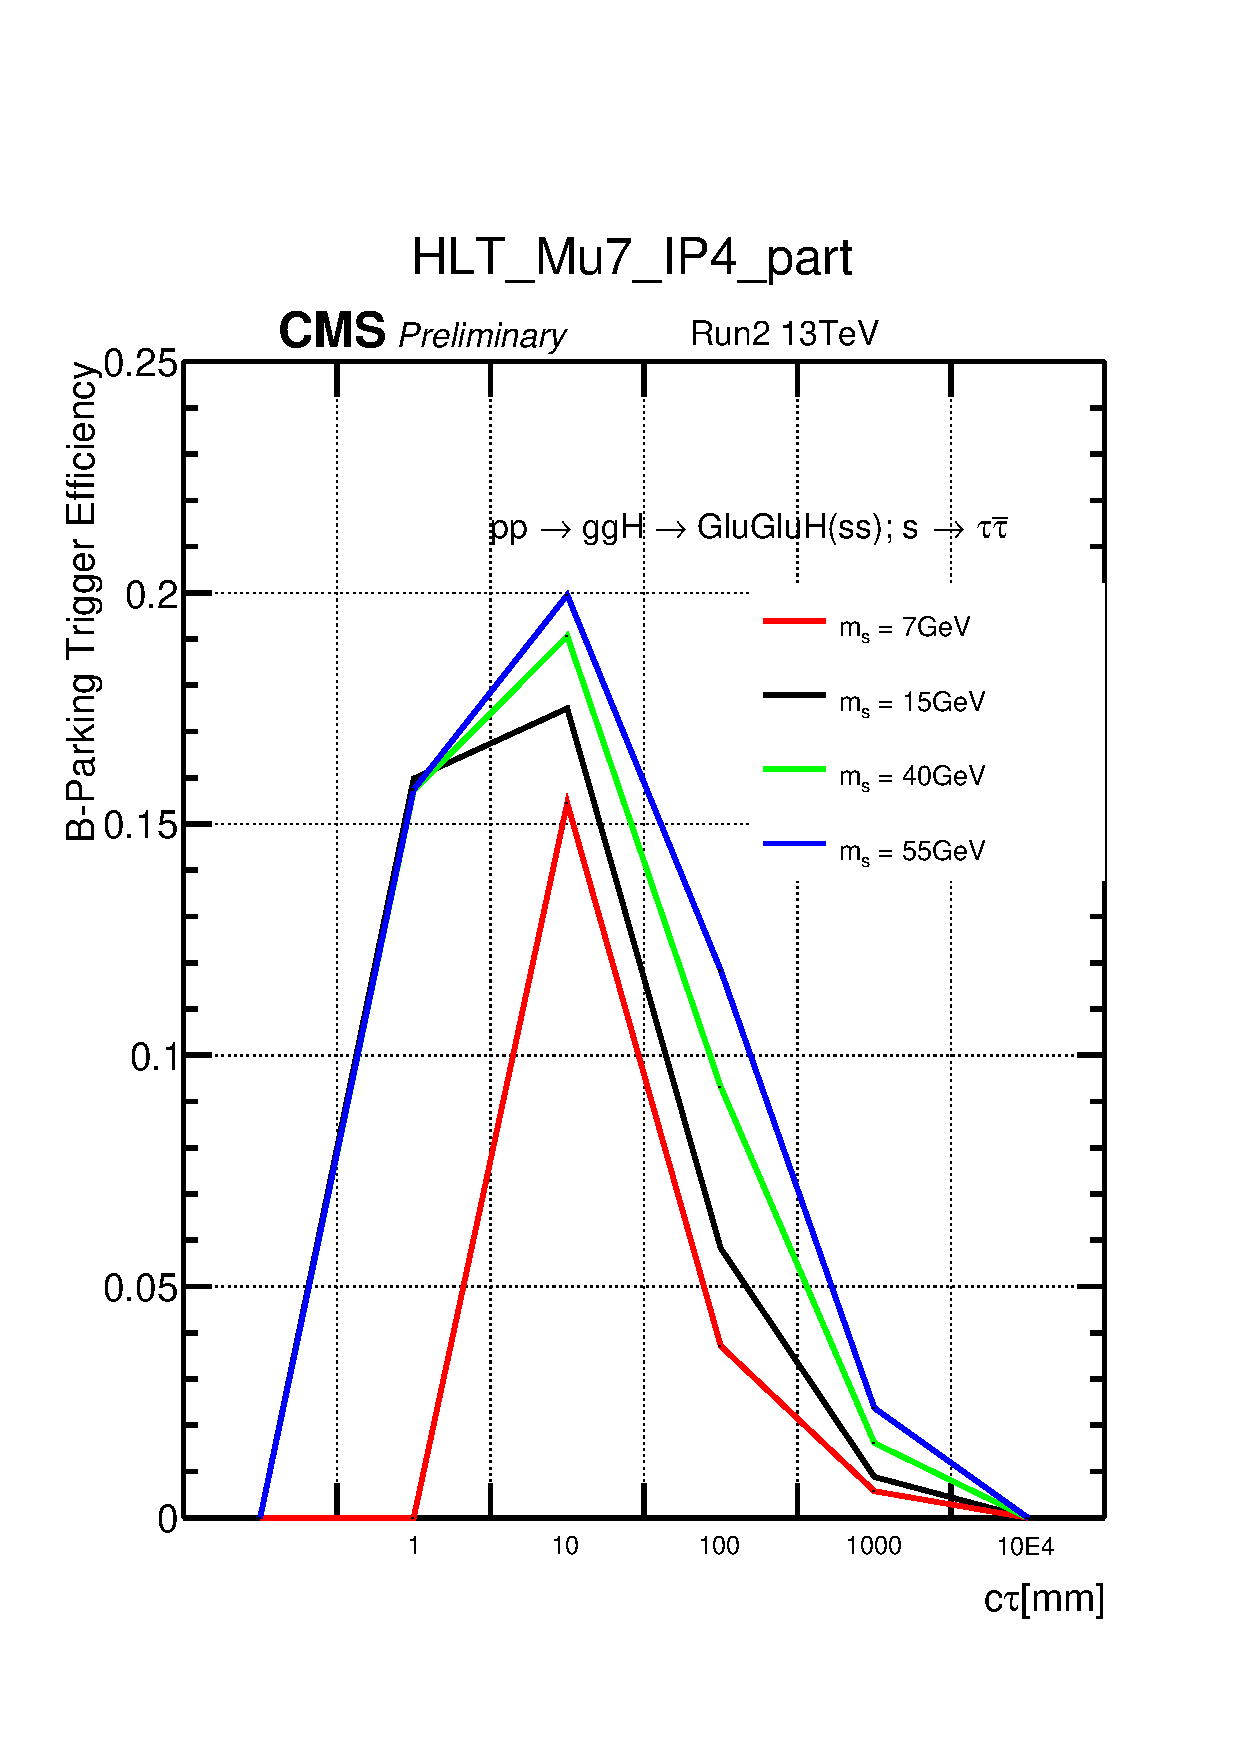
\includegraphics[width=0.47\linewidth]{figs/TrigEff_HLT_Mu7_IP4_part.pdf}
  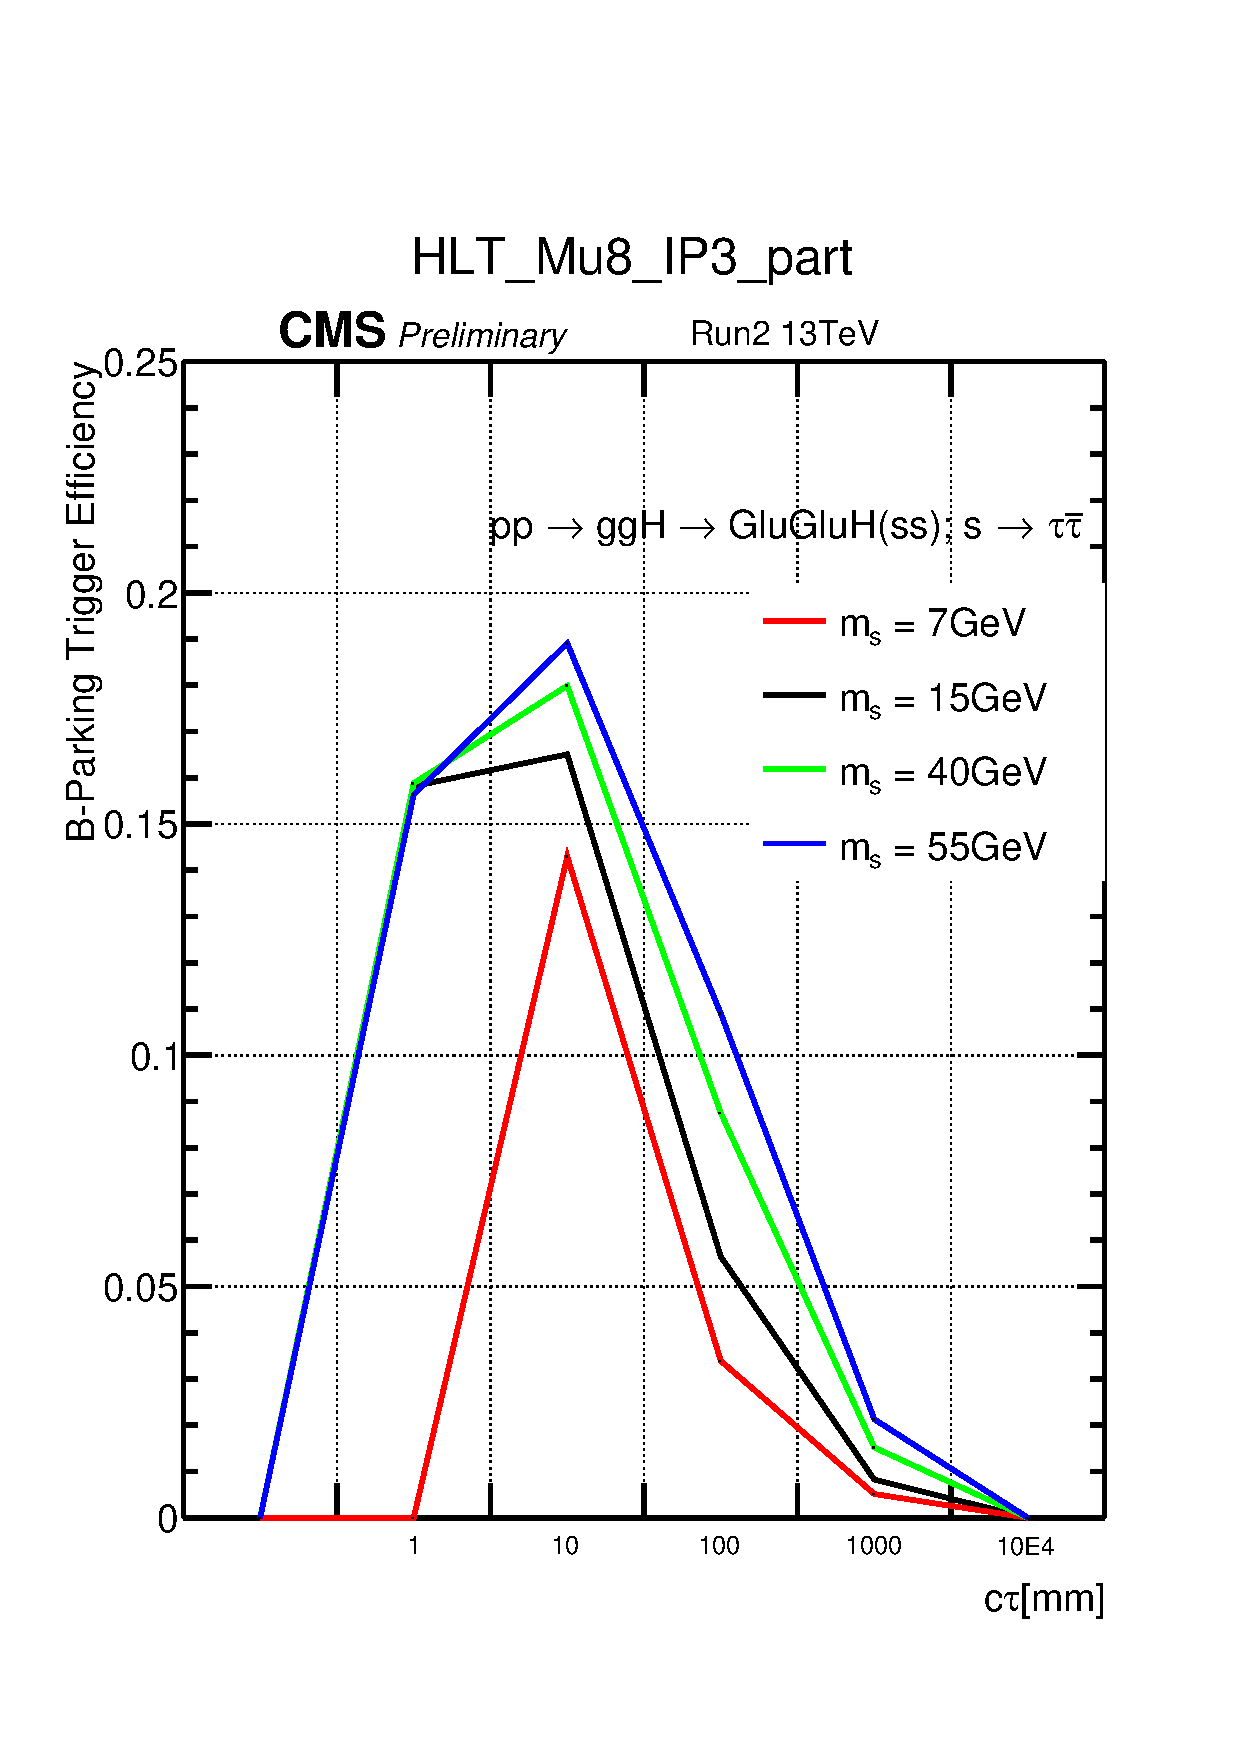
\includegraphics[width=0.47\linewidth]{figs/TrigEff_HLT_Mu8_IP3_part.pdf}

\end{figure}
\begin{figure}[h!]
\caption{Theese plots also show the trigger efficiency for each HLT path with respect to LLP's lifetime. Each line denotes mass scale of each scalar. The analysis uses Mu9\_IP6 for Era A,B of data and Mu12\_IP6 for Era C,D of data}
  \centering
  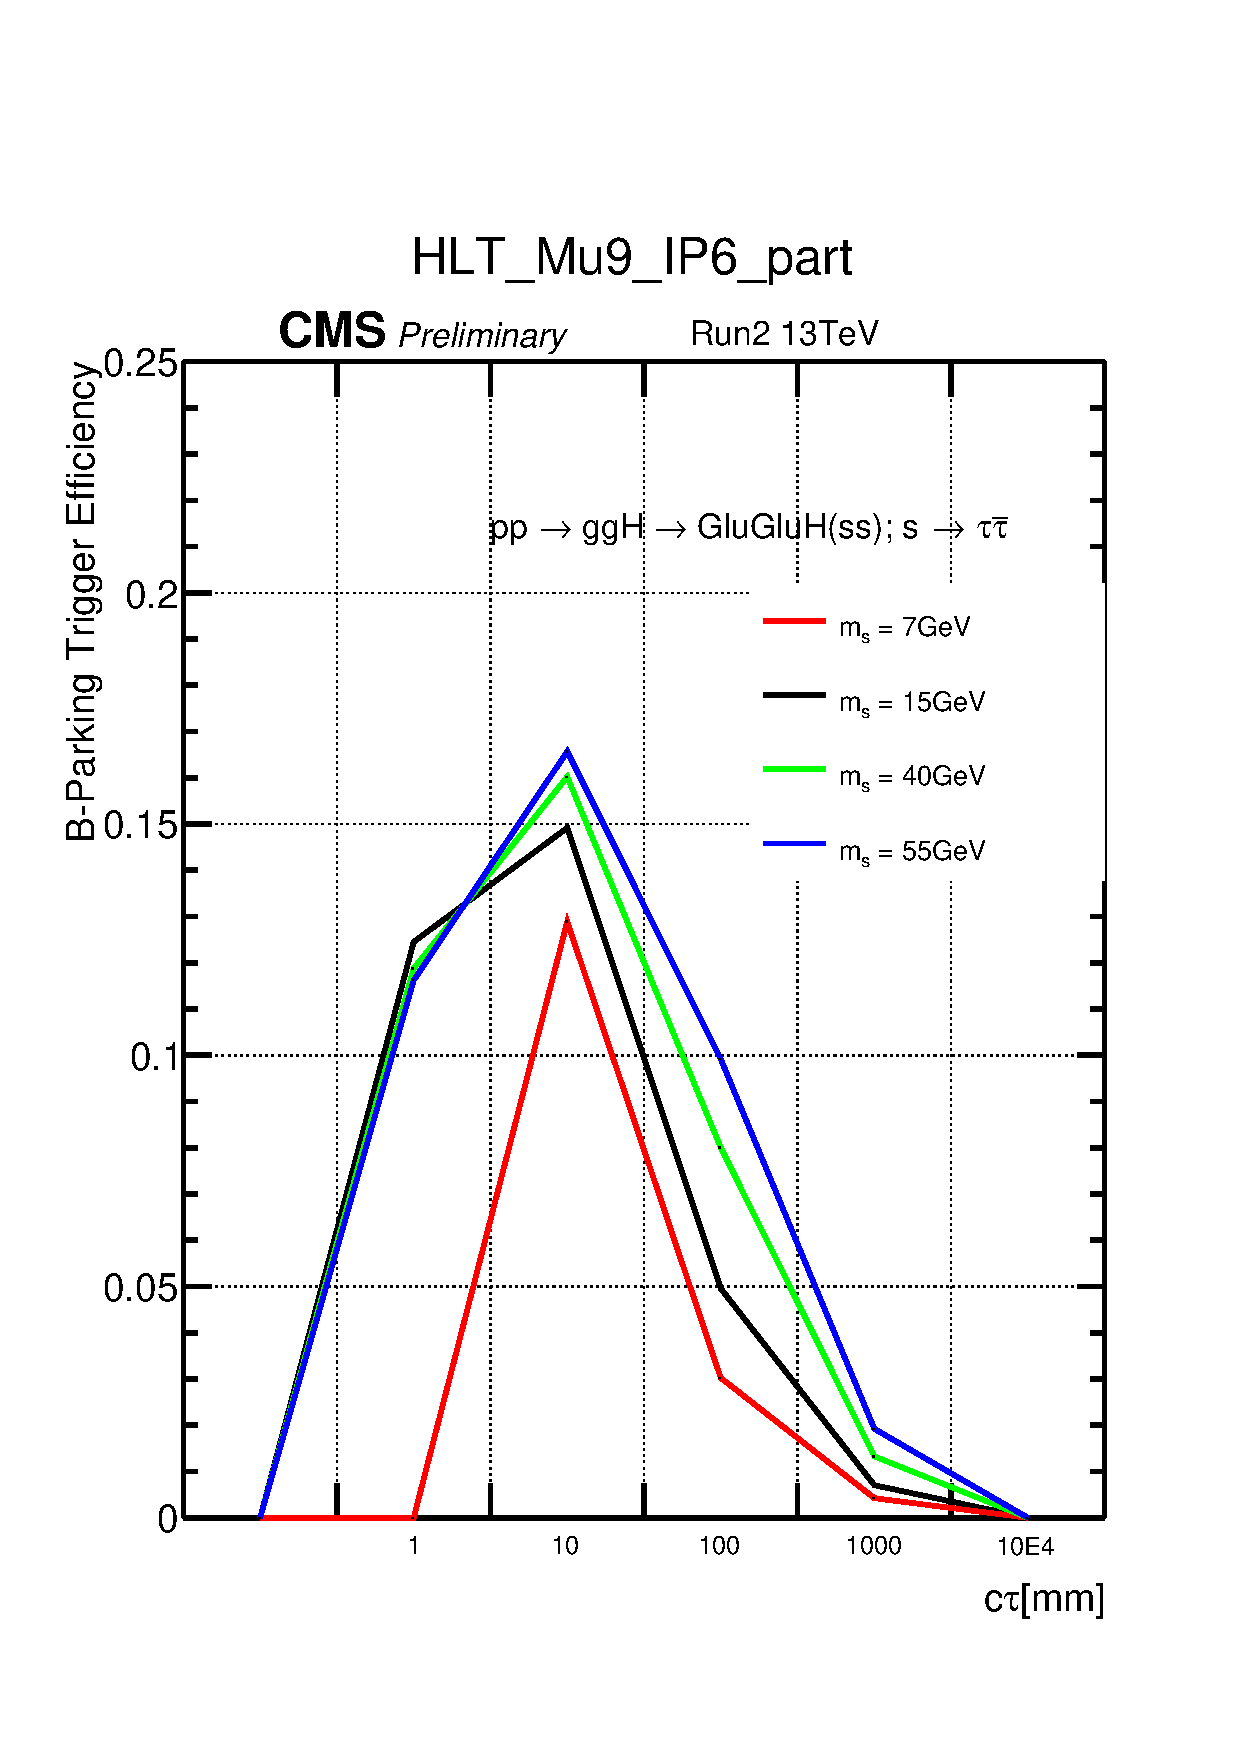
\includegraphics[width=0.47\linewidth]{figs/TrigEff_HLT_Mu9_IP6_part.pdf}
  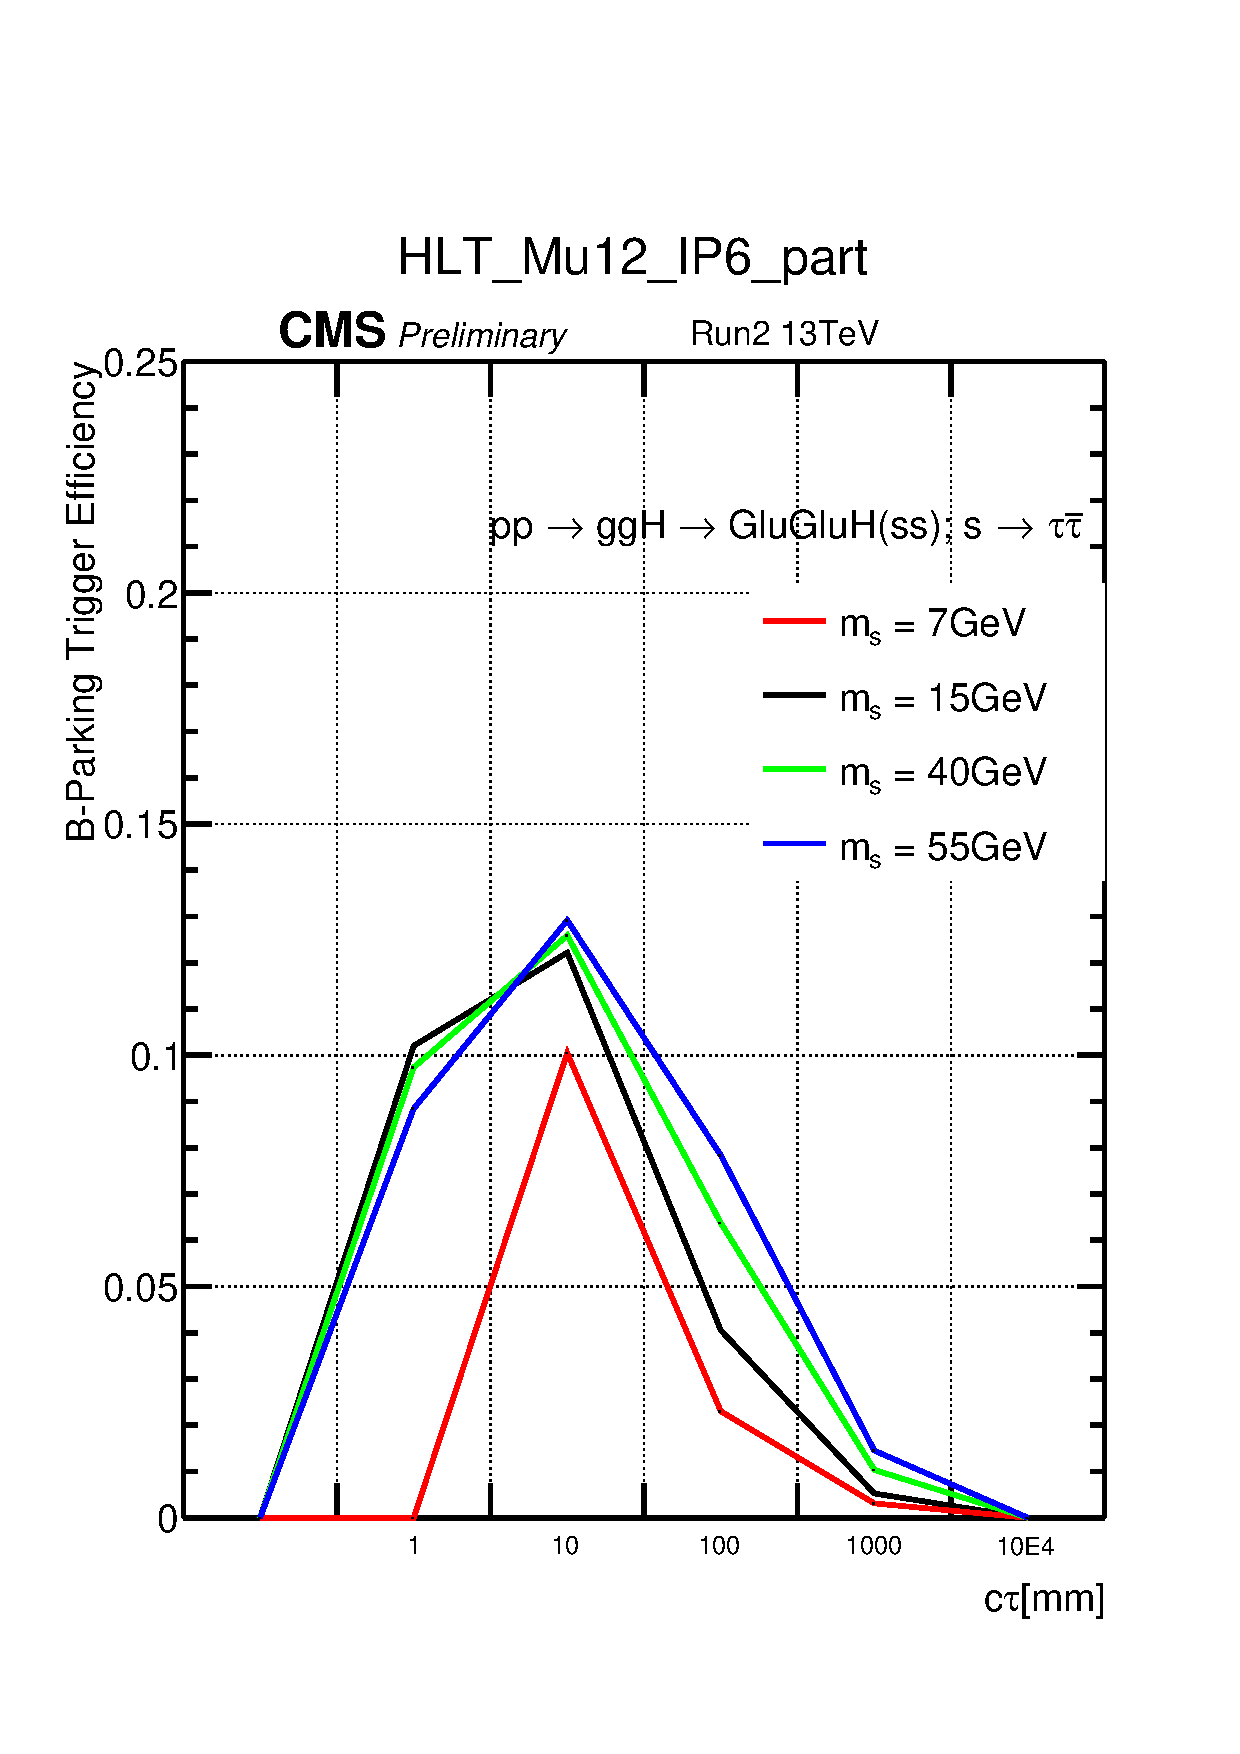
\includegraphics[width=0.47\linewidth]{figs/TrigEff_HLT_Mu12_IP6_part.pdf}

\end{figure}

In contrast to the signal, the background process shows a poor trigger efficiency.
Drell-Yan process and W-Jet process show an even poorer trigger efficiency due to absence of heavy flavor particles in its final state.
TTJets, Single Tops, and QCD-MuEnriched passes the trigger at better efficiency.
All these background processes have heavy flavor particles for its final state (b-quark or top quark).
QCD-MuEnriched has better efficiency for higher Pt bin samples, since higher Pt and HT bin samples tend to have more b-jets for its final state as well.


\section{Integrated Luminosity and pileup weight for the HLT path}

The integrated luminosity for each era has been summarized in table \ref{tab:datasample2018BPH} in Appendix A. 
The information was obtained with commands in section \ref{sec:PU} in Appendix A as well.
The integrated Luminosity totals at 44$fb^{-1}$ lower than 58.7$fb^{-1}$ for the year of 2018 due to prescaling.
The bunch-crossing for B-pakring HLT path is also very different form other HLT paths.
B-parking data are recorded during lower bunch-crossing runs as expected, due to its extreme rate in the CMS collider.

To model Monte Carlo (MC) simulation correctly to describe data, it is vital to adjust this bunch-crossing variable. 
To achieve the purpose, we apply pileup weight on the MC simulation.
Pileup weight is simply a bunch-crossing of data divided by the bunch-crossing of MC for a specific era.
Pileup (PU) weight values are calculated for each era of data-taking (A,B,C,D).
Figure~\ref{fig:EraAData} shows the BPH1-Era A's HLT\_Mu9\_IP6 HLT path's Data PU distribution.
\begin{figure}[h!]
  \caption{Bunch crossing of dataset /ParkingBPH1/Run2018A-UL2018\_MiniAODv2-v1/MINIAOD}
  \label{fig:EraAData}
  \centering
  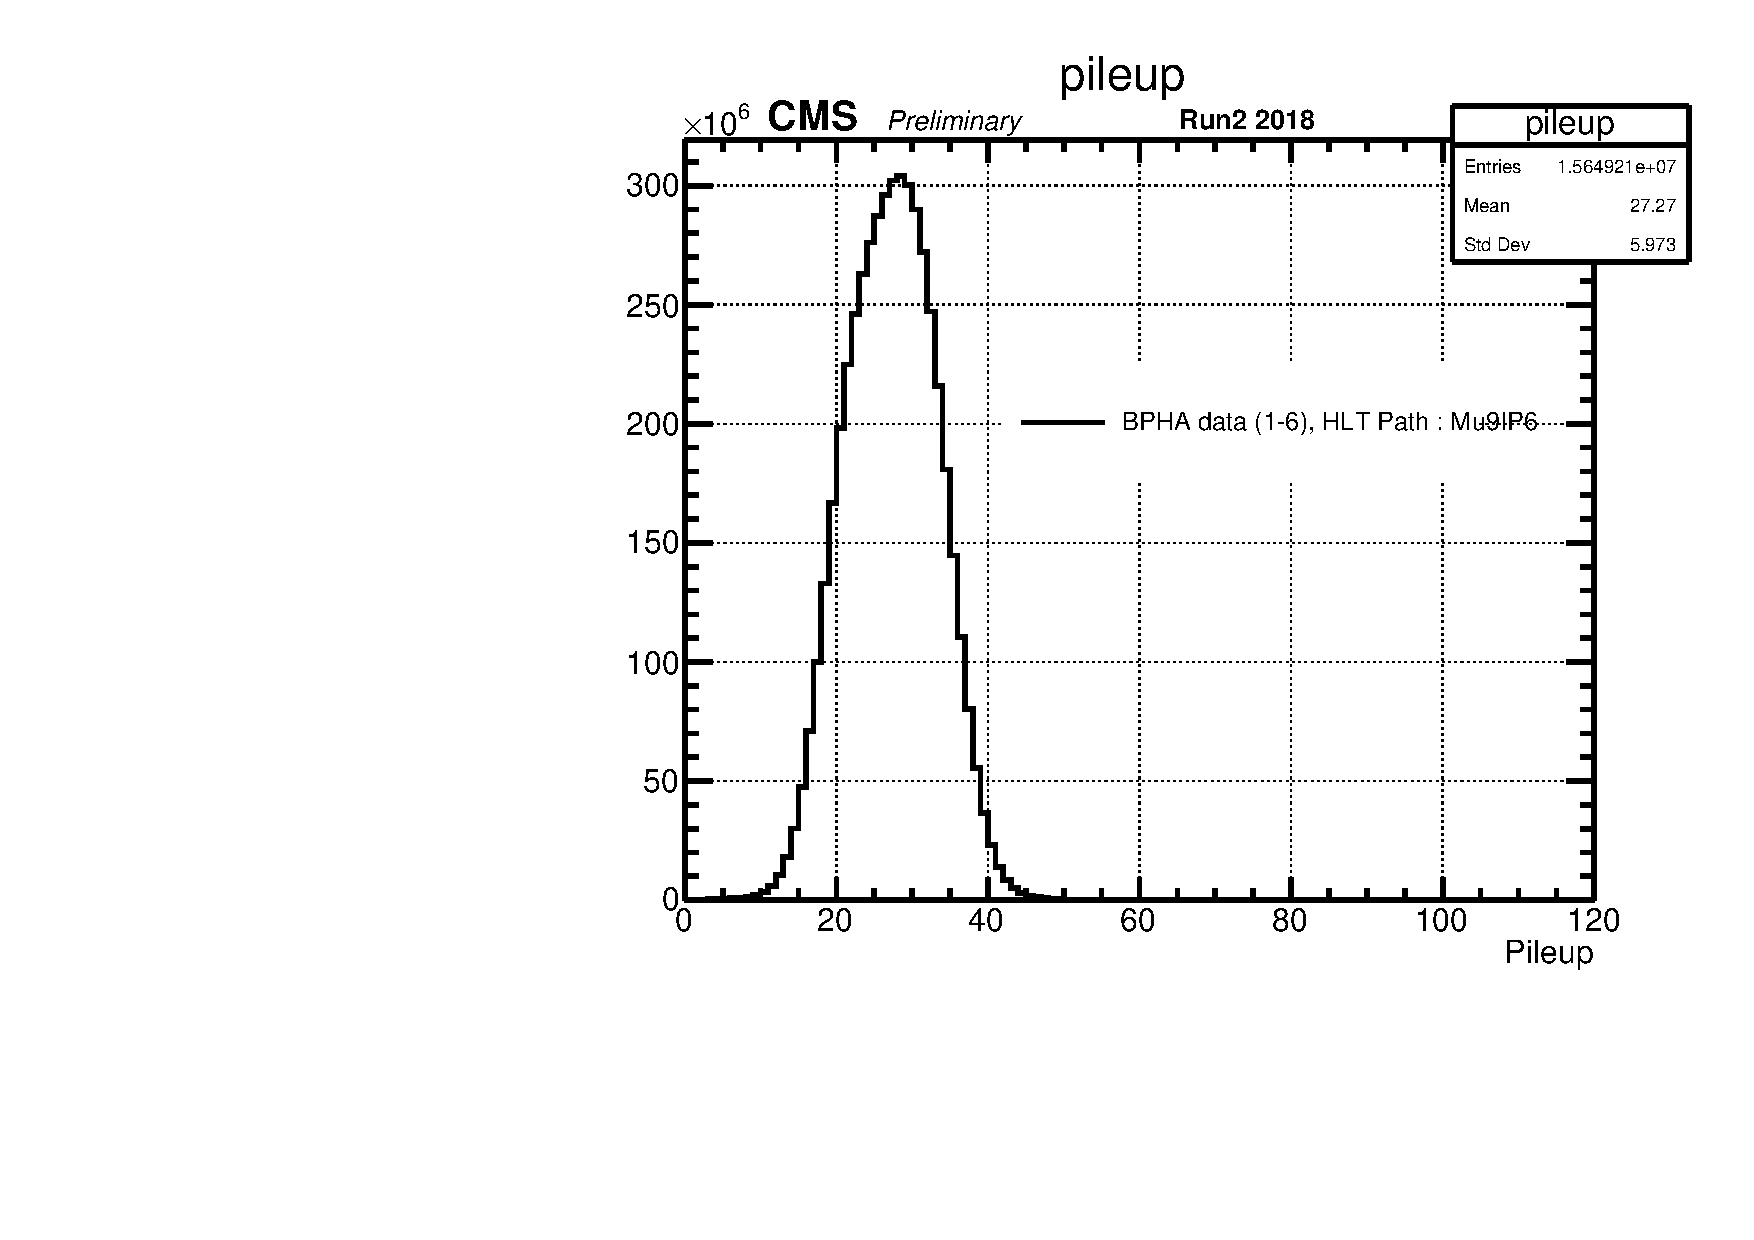
\includegraphics[width=0.67\linewidth]{figs/NVtx_BPHA.pdf}

\end{figure}

Figure~\ref{fig:EraAData} shows the BPH1-Era B's HLT\_Mu9\_IP6 HLT path's Data PU distribution.
\begin{figure}[h!]
  \caption{Bunch crossing of dataset /ParkingBPH1/Run2018B-UL2018\_MiniAODv2-v1/MINIAOD}
  \label{fig:EraAData}
  \centering
  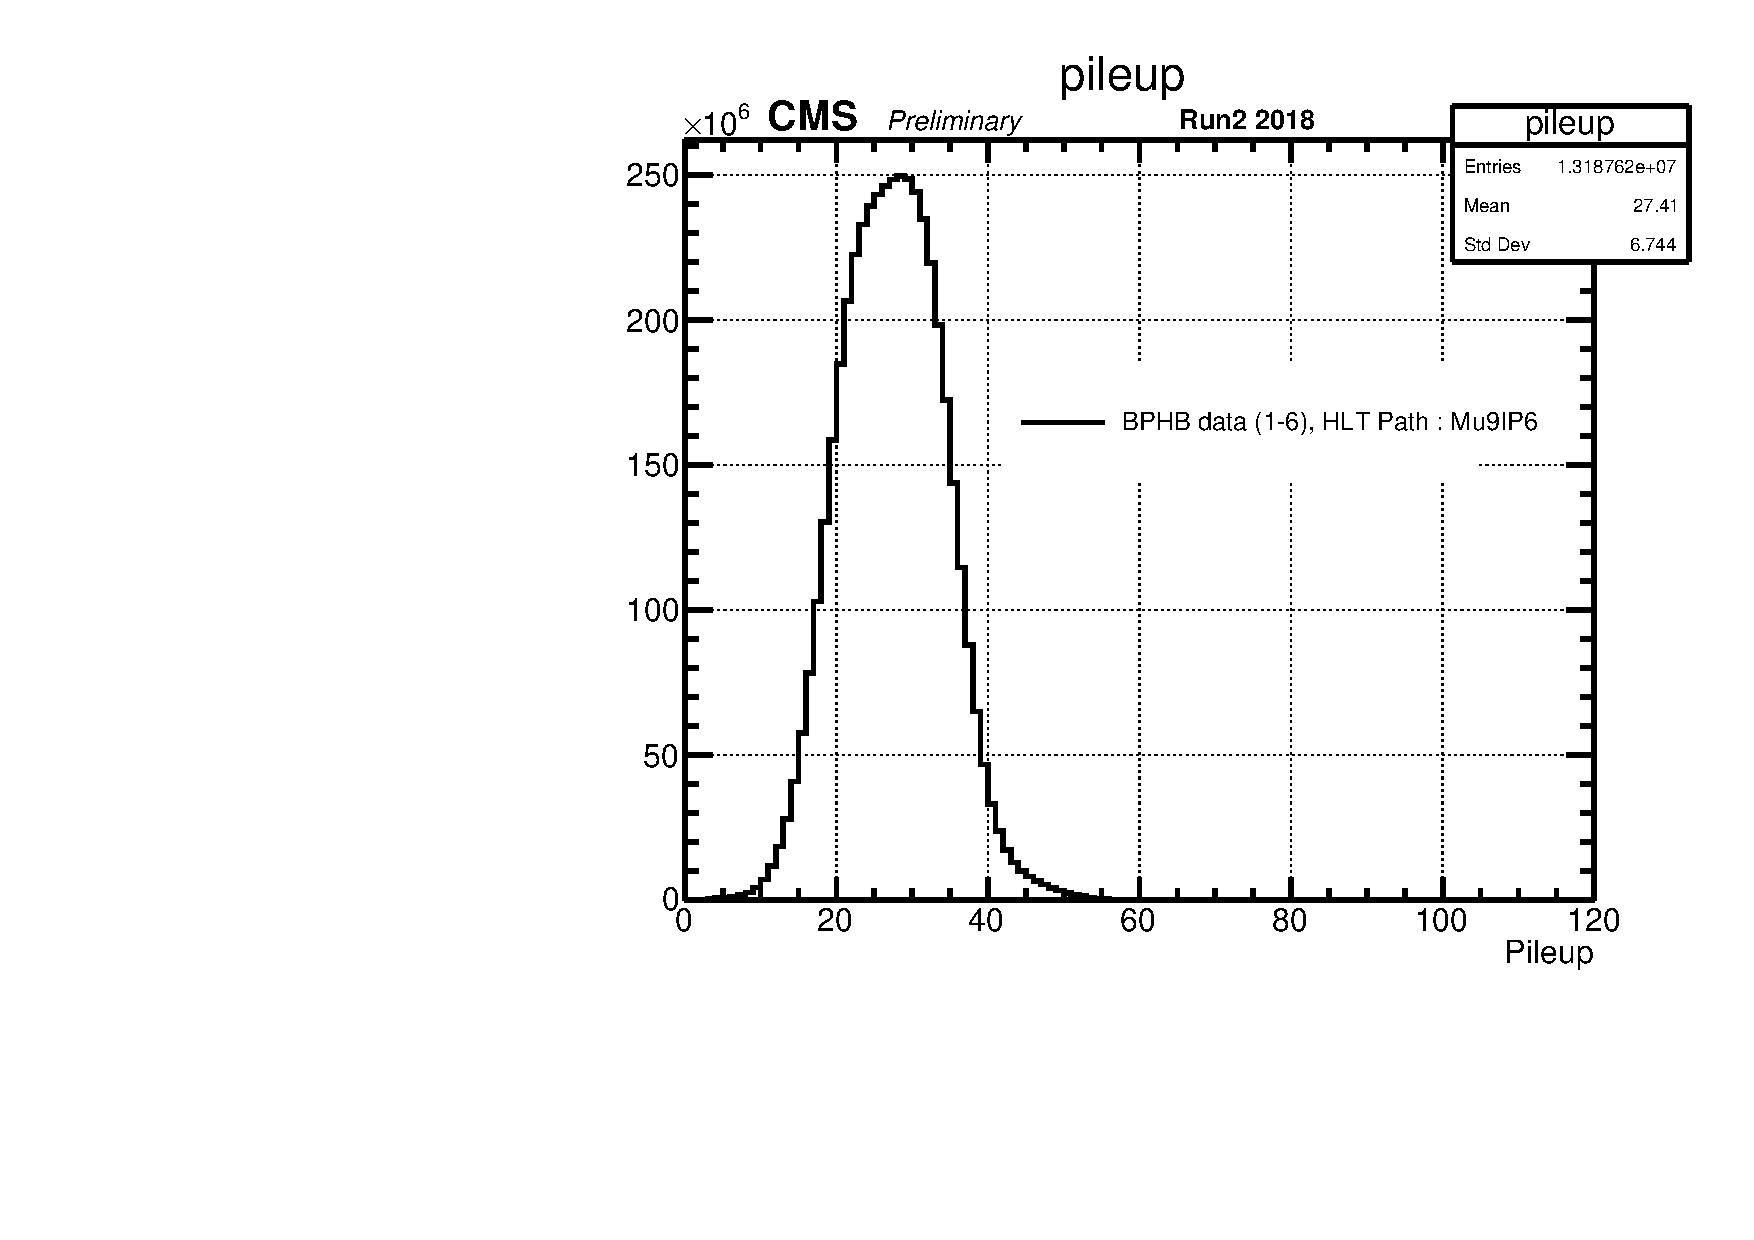
\includegraphics[width=0.67\linewidth]{figs/NVtx_BPHB.pdf}

\end{figure}

Figure~\ref{fig:EraCData} shows the BPH1-Era C's HLT\_Mu12\_IP6 HLT path's Data PU distribution.
\begin{figure}[h!]
\caption{Bunch crossing of dataset /ParkingBPH1/Run2018C-UL2018\_MiniAODv2-v1/MINIAOD. Please note that the HLT path for EraC has higher muon object's pT threshold with 12GeV (compared to 9GeV in EraA).}
  \label{fig:EraCData}
  \centering
  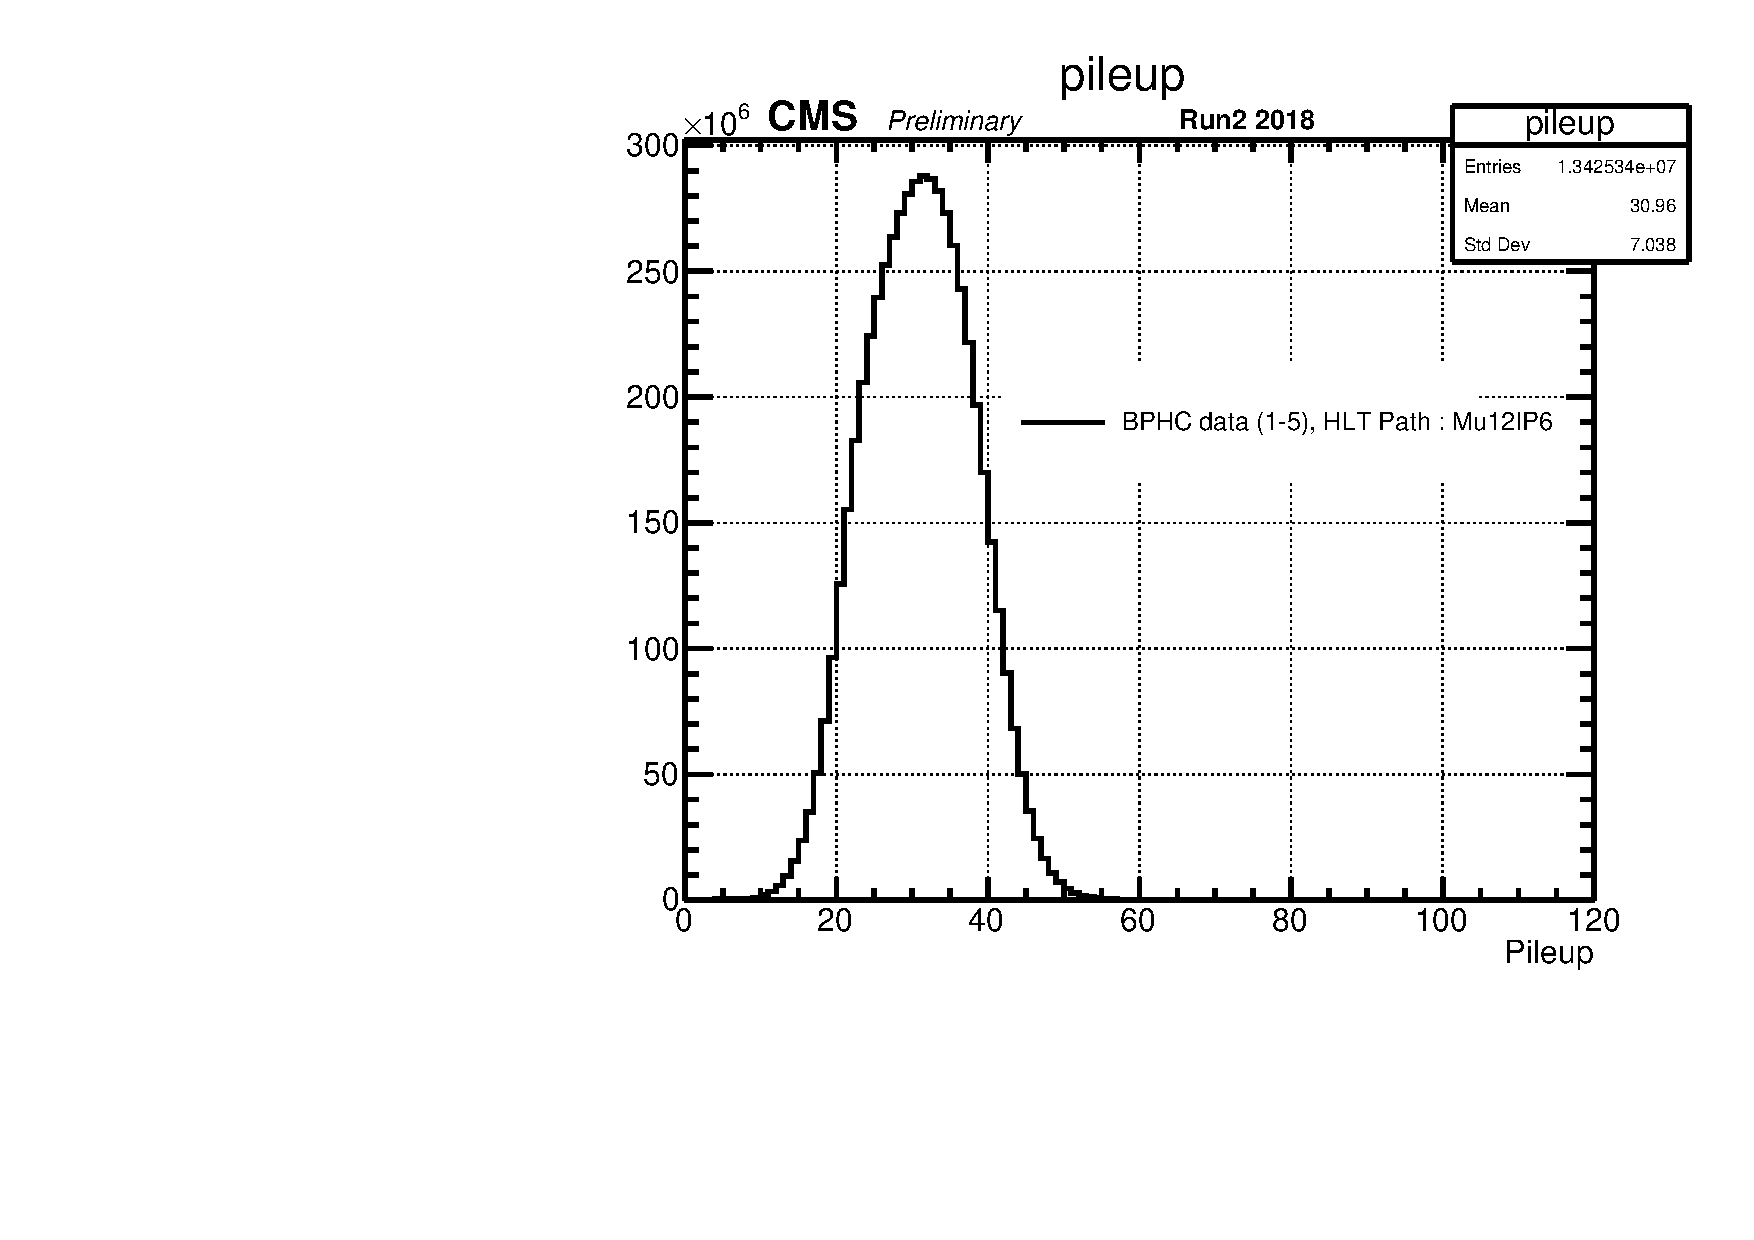
\includegraphics[width=0.57\linewidth]{figs/NVtx_BPHC.pdf}

\end{figure}

Figure~\ref{fig:EraCData} shows the BPH1-Era D's HLT\_Mu12\_IP6 HLT path's Data PU distribution.
\begin{figure}[h!]
\caption{Bunch crossing of dataset /ParkingBPH1/Run2018D-UL2018\_MiniAODv2-v1/MINIAOD. Please note that the HLT path for EraD has higher muon object's pT threshold with 12GeV (compared to 9GeV in EraA).}
  \label{fig:EraCData}
  \centering
  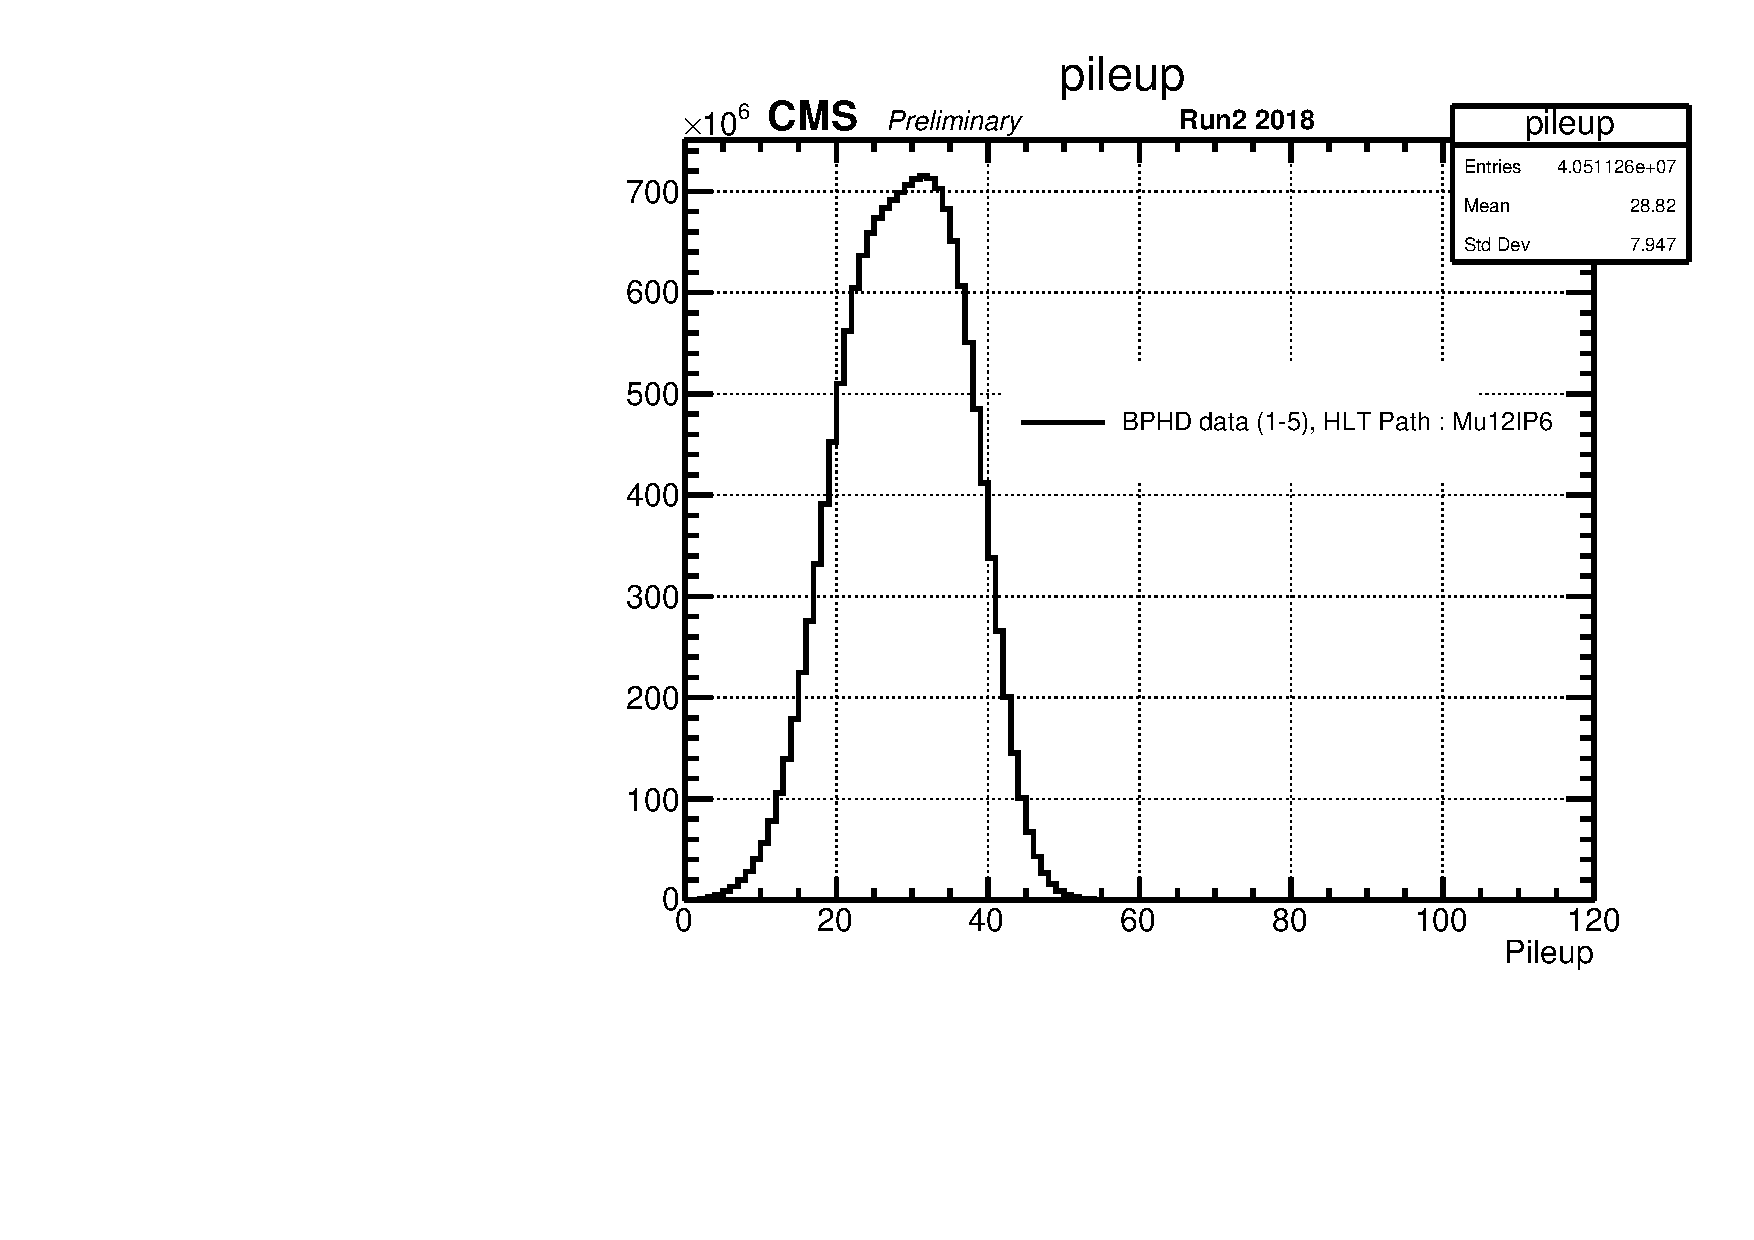
\includegraphics[width=0.57\linewidth]{figs/NVtx_BPHD.pdf}

\end{figure}

Figure~\ref{fig:MCPU} shows DYJetsToLL\_M-50\_TuneCP5\_13TeV-madgraphMLM-pythia8 MC PU distribution.
\begin{figure}[h!]
	\caption{Bunch crossing of Monte Carlo Simulation for physics process of Drell-Yan. The dataset is /DYJetsToLL\_M-50\_TuneCP5\_13TeV-madgraphMLM-pythia8/RunIISummer20UL18MiniAODv2-106X\_upgrade2018\_realistic\_v16\_L1v1-v2/MINIAODSIM}
  \label{fig:MCPU}
  \centering
  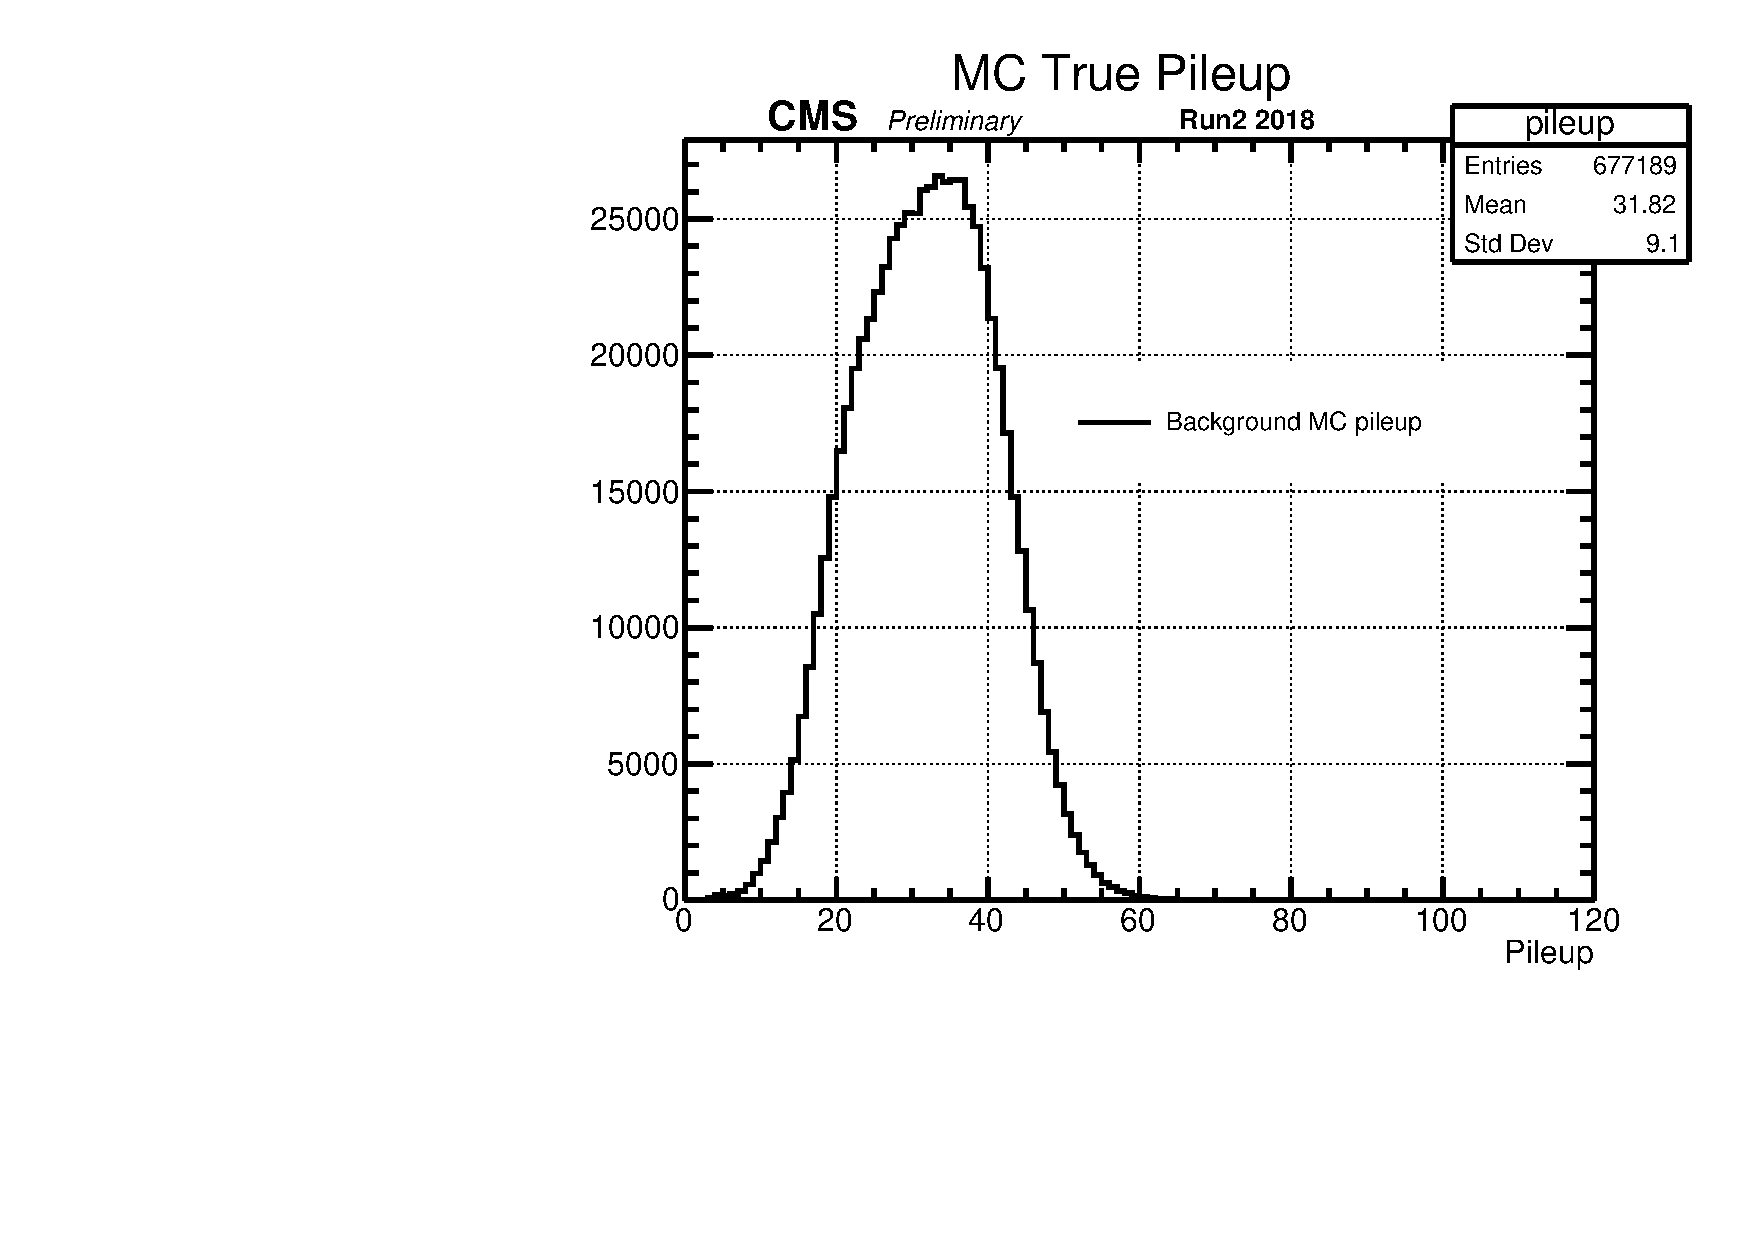
\includegraphics[width=0.67\linewidth]{figs/NVtx_DYJetsToLL_M-50_try.pdf}

\end{figure}

Figure~\ref{fig:PUWeight9} shows resultant such PUWeight from BPH1\_A HLT\_Mu9\_IP6 and DYJetsToLL\_M-50\_TuneCP5\_13TeV-madgraphMLM-pythia8.
\begin{figure}[h!]
  \caption{PUweight calculated for Era A of B-parking dataset}
  \label{fig:PUWeight9}
  \centering
  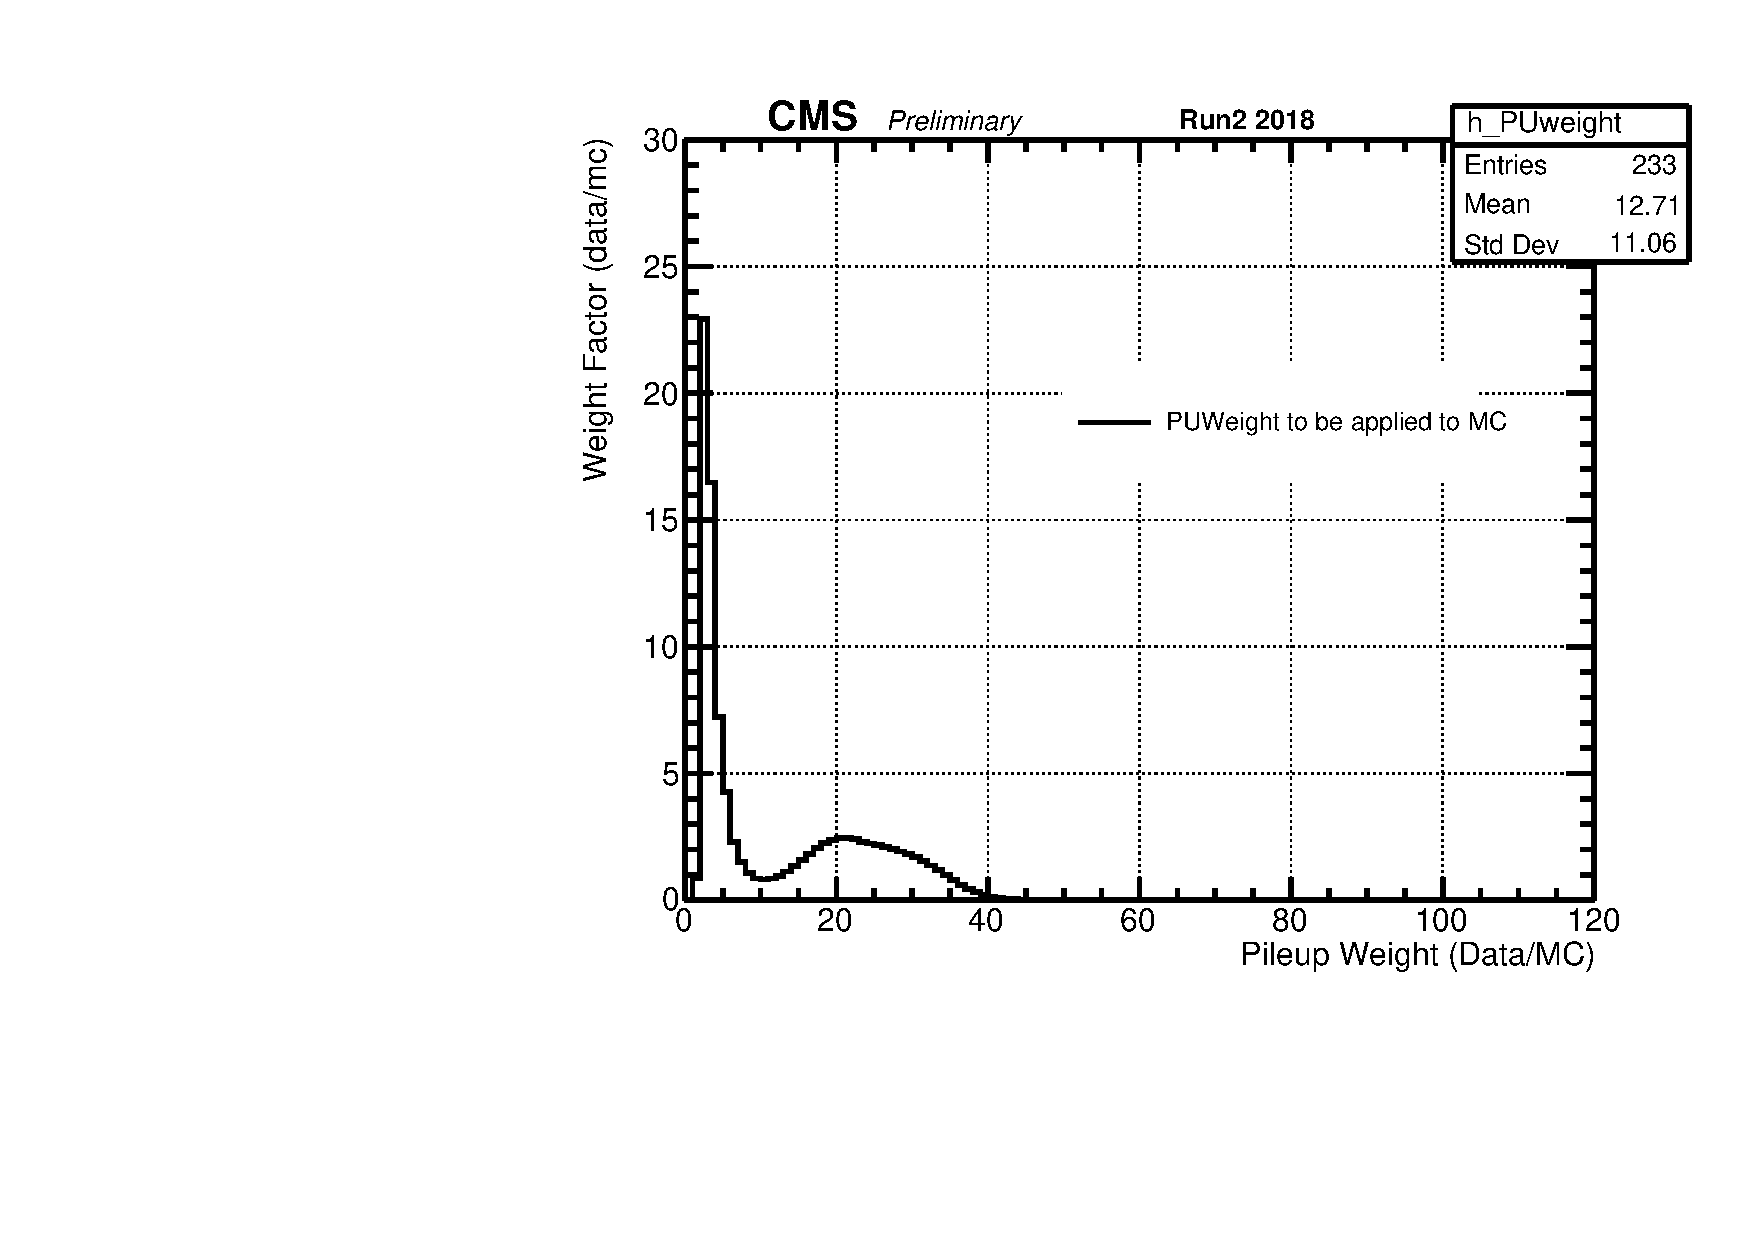
\includegraphics[width=0.67\linewidth]{figs/NVtx_PUWeight.pdf}

\end{figure}
